% ! TeX program = lualatex
\documentclass[a4paper,11pt]{article} 
% packages
\usepackage{censor}
\StopCensoring
\usepackage{fontspec}
\setmainfont{EB Garamond}
% for tironian et fallback
% % \directlua{luaotfload.add_fallback
% % ("emojifallback",
% %      {"Noto Serif:mode=harf"}
% % )}
% % \setmainfont{EB Garamond}[RawFeature={fallback=emojifallback}]

\setmonofont[Scale=MatchLowercase]{Deja Vu Sans Mono}
\usepackage[a4paper,left=2cm,right=2cm,top=\dimexpr15mm+1.5\baselineskip,bottom=2cm]{geometry}
\setlength{\parindent}{0pt}

\usepackage{fancyhdr}       % Headers and footers 
\fancyhead[R]{\normalfont \leftmark}
\fancyhead[L]{}
\pagestyle{fancy}

\usepackage{microtype}      % Slightly tweak font spacing for aesthetics
\usepackage[english]{babel} % Language hyphenation and typographical rules
\usepackage{xcolor}
\definecolor{linkblue}{RGB}{0, 64, 128}
\usepackage[final, colorlinks = false, urlcolor = linkblue]{hyperref} 
% \newcommand{\secref}[1]{\textbf{§~\nameref{#1}}}
\newcommand{\secref}[1]{\textbf{§\ref{#1}~\nameref{#1}}}

\usepackage{changepage}     % adjust margins on the fly

\usepackage{minted}
\usemintedstyle{algol_nu}

\usepackage{pgfplots}
\pgfplotsset{width=\textwidth,compat=1.9}

\usepackage{caption}
\newenvironment{code}{\captionsetup{type=listing}}{}
\captionsetup[listing]{skip=0pt}
\setlength{\abovecaptionskip}{5pt}
\setlength{\belowcaptionskip}{5pt}

\usepackage[yyyymmdd]{datetime}
\renewcommand{\dateseparator}{--}

\usepackage{enumitem}

\usepackage{titlesec}

\author{Andrew Hayes}

\begin{document}
\begin{titlepage}
    \begin{center}
        \hrule
        \vspace*{0.6cm}
        \Huge \textsc{ct3532}
        \vspace*{0.6cm}
        \hrule
        \LARGE
       \vspace{0.5cm}
       Assignment 3: Graphs
       \vspace{0.5cm}
       \hrule

       \footnotesize
       \vfill
        % \begin{figure}[H]
            \centering
            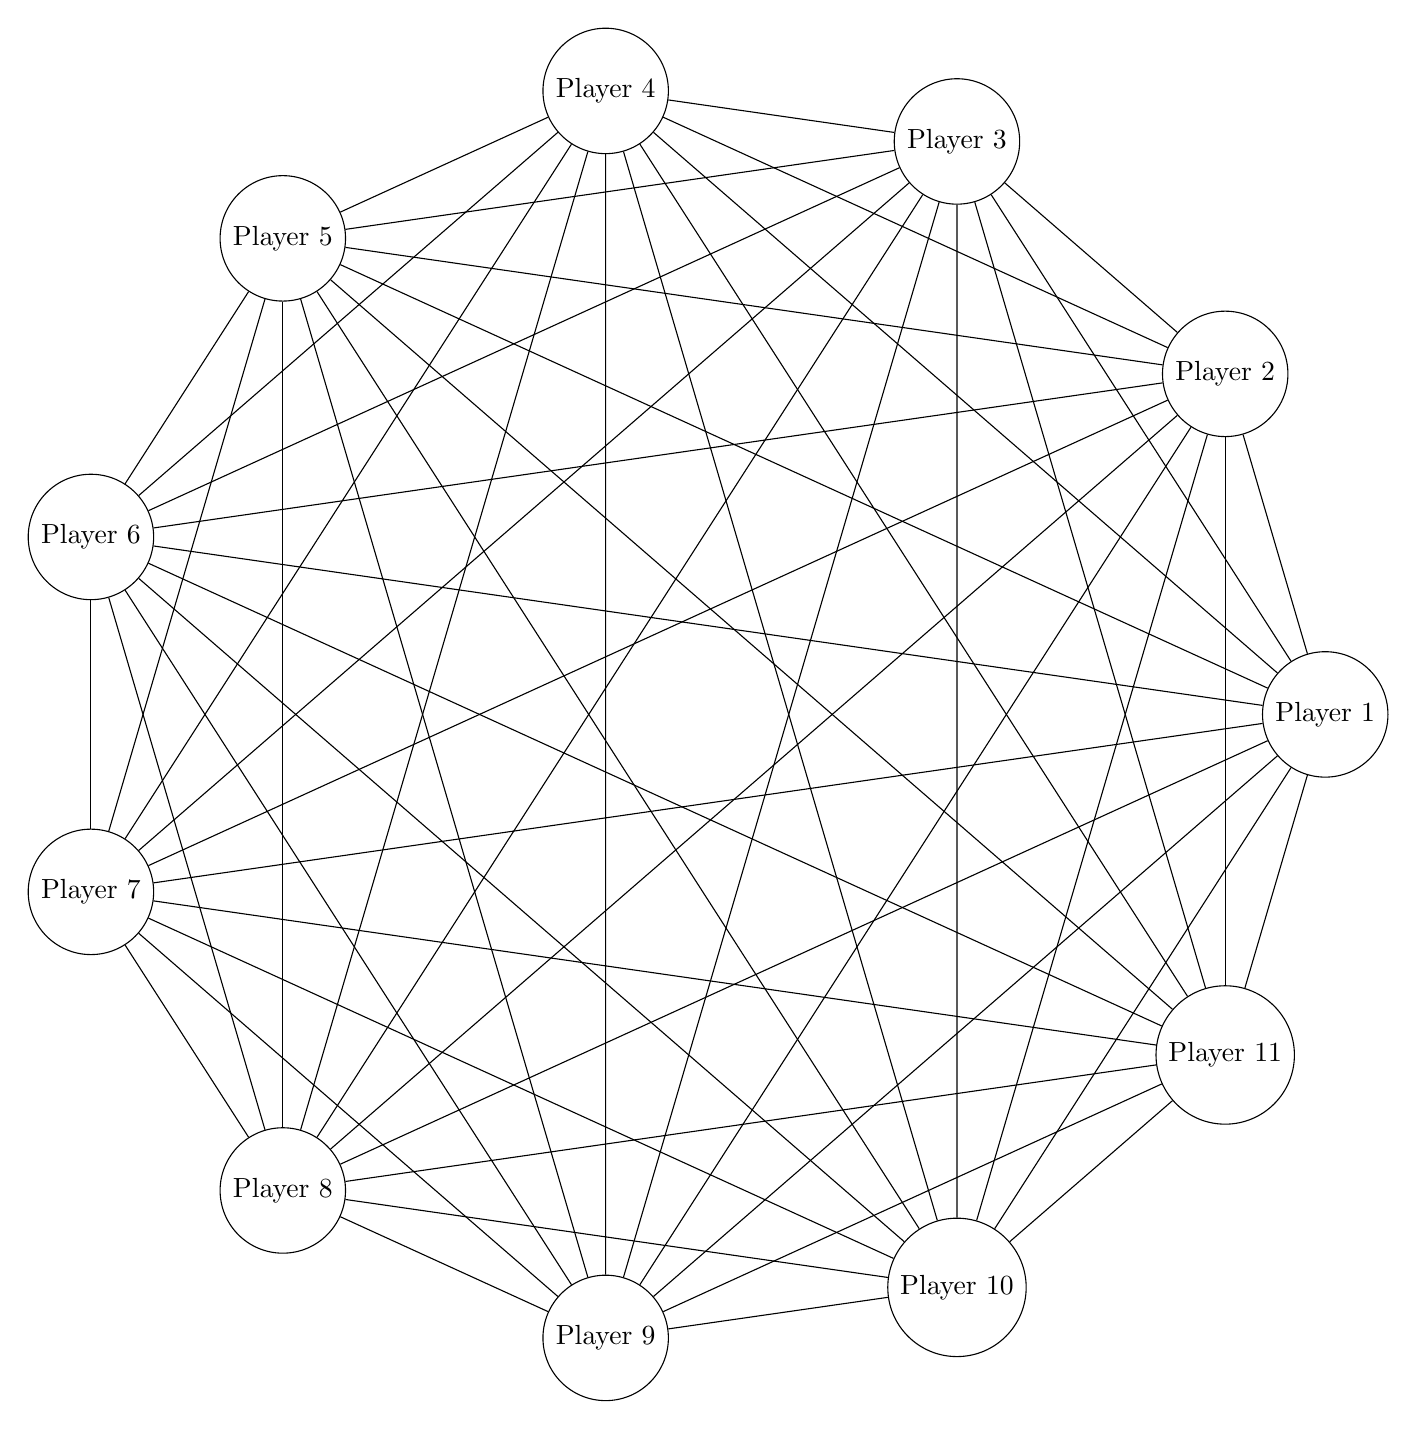
\begin{tikzpicture}
              % Define the nodes
              \foreach \x in {1,...,11}
                \node[circle,draw] (node\x) at ({360/11 * (\x - 1)}:8) {Player $\x$};

              % Define the edges and their distances
              \foreach \i in {1,...,11} {
                \foreach \j in {\i,...,11} {
                  \ifnum\i=\j\relax
                  \else
                    % \pgfmathsetmacro\distance{rand} % Generate random distances
                    % \draw (node\i) -- (node\j) node[midway, sloped, above] {\distance};
                    \draw (node\i) -- (node\j) ;
                  \fi
                }
              }
            \end{tikzpicture}
            % \caption{An Example Graph with 11 Nodes Representing a Team}
        % \end{figure}
       \vfill

       % \vspace{1.6cm}
       \hrule
        \begin{minipage}{0.495\textwidth} 
            \vspace{0.4em}
            \raggedright
            \normalsize 
            \begin{tabular}{@{}l l}
                Name: & Andrew Hayes \\
                Student ID: & 21321503 \\
                E-mail: & \href{mailto://a.hayes18@universityofgalway.ie}{a.hayes18@universityofgalway.ie} \\
            \end{tabular}
        \end{minipage}
        \begin{minipage}{0.495\textwidth} 
            \raggedleft
            \vspace*{0.8cm}
            \Large
            \today
            \vspace*{0.6cm}
        \end{minipage}
        \medskip\hrule 
    \end{center}
\end{titlepage}

% \title{Report Template}
% \maketitle

\pagenumbering{roman}
\newpage
\tableofcontents
\newpage
\setcounter{page}{1}
\pagenumbering{arabic}

\section{Representing the Graph in a Relational Database}
% \begin{figure}[H]
%     \centering
%     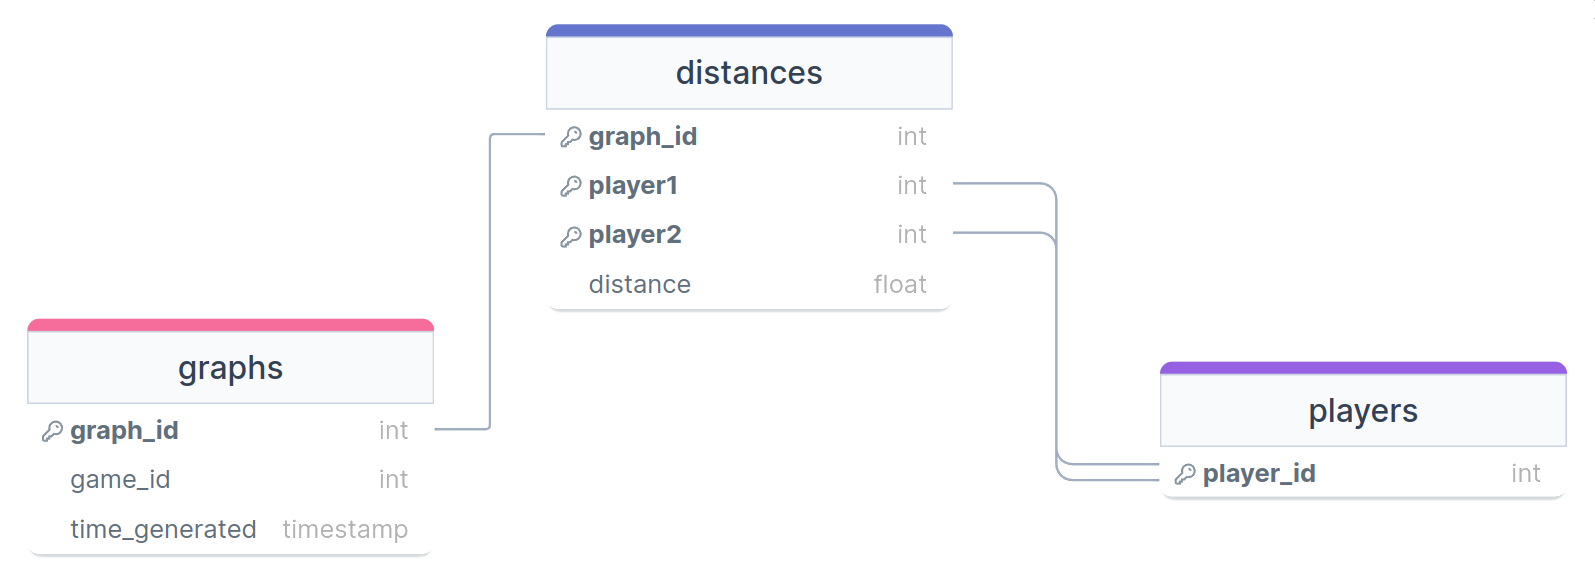
\includegraphics[width=0.8\textwidth]{./images/schema.png}
%     \caption{Database Schema Diagram}
% \end{figure}


The key challenge with representing a complete graph in a database is the number of edges on each node. 
If we take an 11-player soccer team for example, each node will have 10 edges (one joining it to each other node), resulting in a graph like the example 
graph shown on the cover page.
We also need to take into consideration that each edge has distance information associated with it, but no direction 
information.
This means that storing the edges within the node somehow is not a good idea:
since there is no direction information, we would have to decide arbitrarily which node to store an edge with, or duplicate it across both nodes. 
Furthermore, it is not easy to say with certainty the number of edges that we will wish to store for each node at any given time, making it difficult to represent them as, say, 10 distinct columns in a 
table. 
For example, if a player gets sent off and there are no other players available to be substituted in their place, suddenly each node would have only 9 edges, or if we decided that we weren't interested in
storing an edge if the distance between the players was too great to be meaningful, the number of edges stored per node would be variable.
I make the assumption that the graphs in questions are not multigraphs, i.e. there can be no edge joining a node to itself (I can't think of what that would even 
mean in this context, as the distance from a player to themselves would naturally always be 0).
\\\\
My proposed approach for representing the graph in a relational database is to have separate node \& edge tables.
Because each node represents a player and each edge represents the distance between two players, the tables will be named 
\mintinline{sql}{players} \& \mintinline{sql}{distances} respectively to relate them easily to the physical reality that they represent.
We must also consider that the graph may be generated several times throughout a game, so we should be able to distinguish which entries in a given table pertain to which graphs. 
For this reason, I will also make use of a third table called \mintinline{sql}{graphs}, which every entry in the \mintinline{sql}{distances} table will have a foreign key to, allowing us to identify the
graph to which that entry pertains. 

\subsection{The \texttt{graphs} Table}
The \mintinline{sql}{graphs} table will be used to identify each graph. 
The table will have three columns:
\begin{itemize}
    \item   An auto-incrementing integer column called \mintinline{sql}{graph_id} which will serve as the table's primary key. 
            This key will be referenced by each row in the \mintinline{sql}{distances} table so that the graph to which the data in the row relates can be identified.
            An auto-incrementing ID was chosen as opposed to a composite key of the game's ID \& the time of the graph's generation so as to reduce the duplication of data across tables.

    \item   An integer column called \mintinline{sql}{game_id} which uniquely identifies the game to which the graph pertains.
            We assume that this is defined elsewhere, either in a \mintinline{sql}{games} table or simply on an iterative basis, where the $n\textsuperscript{th}$ game played gets a
            \mintinline{sql}{game_id} of $n$.
            The SQL code examples will make the assumption that a \mintinline{sql}{games} table exists, but since this table is irrelevant to the representation of the graph and could be easily done 
            without, I won't bother defining what columns it should contain or how to create it; the only column that it must contain is a \mintinline{sql}{game_id}.
    
    \item   A \mintinline{sql}{TIMESTAMP} column called \mintinline{sql}{time_generated} which represents the time at which the graph was generated. 
            I opted to use a standard \mintinline{sql}{TIMESTAMP} instead of a variable representing the amount of game time that has elapsed for the sake of simplicity \& flexibility.
            This column would constitute a candidate key if there was a guarantee that no two matches would be played simultaneously, and therefore we wouldn't need the \mintinline{sql}{graph_id} or 
            \mintinline{sql}{game_id}. 
            However, I feel that this would be an unreasonable assumption to make and would result in a less robust schema so I opted for the two extra columns instead.
\end{itemize}

\subsubsection{SQL Code to Create the \texttt{graphs} Table}
\begin{code}
\begin{minted}[linenos, breaklines, frame=single]{sql}
CREATE TABLE graphs (
    graph_id INT NOT NULL AUTO_INCREMENT,
    game_id INT NOT NULL,
    time_generated TIMESTAMP NOT NULL,

    PRIMARY KEY (graph_id),
    FOREIGN KEY (game_id) REFERENCES games(game_id) -- assuming that a `graphs` table exists elsewhere 
)
\end{minted}
\caption{SQL Code to Create the \texttt{graphs} Table}
\end{code}

\subsection{The \texttt{players} Table}
The details of the player table depend on what kind of data we want to store per node. 
I am operating under the assumption that we do not intend on storing the $(x,y)$ co-ordinates of the player for each node on the graph. 
This allows us to use some arbitrary \mintinline{sql}{players} table which contains whatever information we want to store on each player such as name, age, team, etc.
The specifics of what is stored in the \mintinline{sql}{players} table are largely irrelevant to the implementation of my schema, the only requirement is that there is an unique integer player ID for 
each player that is unique across teams and games.
For this reason, I will operate with the most bare-bones possible player table which will contain an auto-incrementing integer player ID and nothing else, but in a practical scenario this table ought to 
include columns such as the name of the team to which the player belongs, the player's name, the player's squad number, etc.
\\\\
If, however, we wanted to store the $(x,y)$ co-ordinates of each player with each node, it would be best to not use the \mintinline{sql}{players} table to represent the nodes; instead we should define a 
\mintinline{sql}{nodes} table which has a foreign key to the \mintinline{sql}{players} table, a foreign key to the \mintinline{sql}{graphs} table, \& the $(x,y)$ co-ordinates of the player at the time 
when the graph was generated.

\subsubsection{SQL Code to Create the \texttt{players} Table}
\begin{code}
\begin{minted}[linenos, breaklines, frame=single]{sql}
CREATE TABLE players (
    player_id INT NOT NULL AUTO_INCREMENT,
    -- whatever other relevant information for each player should be included here

    PRIMARY KEY (player_id)
)
\end{minted}
\caption{SQL Code to Create the \texttt{players} Table}
\end{code}

\subsection{The \texttt{distances} Table}
The purpose of the \mintinline{sql}{distances} table is to represent the edges between each pair of nodes. 
It must store the IDs of two nodes (or players) and the distance between them. 
However, since each edge is undirected, there is no easy way to say which node should be stored in which column of the table.
To ensure that the ordering of the node pairs remains consistent, I will store the node with the lower player ID in the first column and the node with the higher player ID in the second column. 
The graph will consist of three columns:
\begin{itemize}
    \item   The \mintinline{sql}{graph_id} of the graph to which this edge belongs, which will reference the \mintinline{sql}{graphs} table. 

    \item   A column named \mintinline{sql}{player1} which will hold the player ID of the first player in the pair of nodes that the edge joins. 
            The player ID stored in this column will be the lesser of the two player IDs in question, so that we can ensure that the ordering remains consistent.
            This column will be a foreign key that references the \mintinline{sql}{players} table.

    \item   A column named \mintinline{sql}{player2} which will hold the player ID of the second player in the pair of nodes that the edge joins. 
            The player ID stored in this column will be the greater of the two player IDs in question, so that we can ensure that the ordering remains consistent.
            This column will also be a foreign key that references the \mintinline{sql}{players} table.

    \item   A column named \mintinline{sql}{distance} which will store the distance between the two players at the time the graph was generated.
            Assuming that this is measured in metres or some similar unit, this column will need to be a floating point number.
\end{itemize}

Because I don't expect to have any foreign keys referencing this table, it is likely more efficient in terms of space to use a composite key comprised of the columns \mintinline{sql}{graph_id},
\mintinline{sql}{player1}, \& \mintinline{sql}{player1} instead of having an auto-incrementing \mintinline{sql}{distance_id} column.

\subsubsection{SQL Code to Create the \texttt{distances} Table}
\begin{code}
\begin{minted}[linenos, breaklines, frame=single]{sql}
CREATE TABLE distances (
    graph_id INT NOT NULL,
    player1 INT NOT NULL,
    player2 INT NOT NULL,
    distance FLOAT,

    PRIMARY KEY (graph_id, player1, player2),
    FOREIGN KEY (graph_id) REFERENCES graphs(graph_id),
    FOREIGN KEY (player1) REFERENCES players(player_id),
    FOREIGN KEY (player2) REFERENCES players(player_id),
)
\end{minted}
\caption{SQL Code to Create the \texttt{distances} Table}
\end{code}

\section{Representing the Data in a Data Structure} \label{sec:data_structure}
One of the most obvious ways to represent this data in a data structure (to me, at least) is to take an object-oriented programming approach.
My proposed data structure would be a hierarchy in which objects would be encapsulated within other objects.
There would be a class of \mintinline{java}{Game} objects which would contain all the data related to a game, including a set of \mintinline{java}{Graph} objects. 
These \mintinline{java}{Graph} objects would contain all the data related to a graph generated at a moment in time during the game, including a timestamp of when the graph was generated and a set of 
\mintinline{java}{Edge} objects.
Each of these \mintinline{java}{Edge} objects would contain two \mintinline{java}{Player} objects and the distance between them. 
Finally, the \mintinline{java}{Player} objects would each contain data about the player which they represent, such as name, team name, etc.
The \mintinline{java}{Player} objects would be contained within the \mintinline{java}{Edge} objects using an unordered set, as the edges are undirected.
The choice to store \mintinline{java}{Player} (node) objects inside \mintinline{java}{Edge} objects instead of vice-versa is because the number of nodes per edge 
is known to always be 2, whereas a node could have as many edges as there are other nodes in the graph.
\\\\
An obvious question that arises from this proposed data is one of data duplication: if each edge contains two players, would that not mean that each player object is duplicated for every edge object 
between it and another player? 
We can avoid duplicating data by representing this data structure in a language such as Java, as Java allows us to make reference to objects within several different objects, using what is essentially a 
data pointer.
Therefore, two (or 10) \mintinline{java}{Edge} objects could make reference to the same \mintinline{java}{Player} object without duplicating the data contained within that \mintinline{java}{Player} object.

\subsection{Code to Represent the Data in a Data Structure}\label{sec:data_structure_code}
The following (highly simplified) Java code could be used to represent the proposed classes:
\begin{code}
\begin{minted}[texcl, mathescape, linenos, breaklines, frame=single]{Java}
// Note that in Java, there can be only one `public` class per file
// Therefore, if this code were to be actually used, each class must be in its own `*.java` file

public class Game {
    // potential data fields that could be contained within the Game class
    public int gameId;
    public String homeTeam;
    public String awayTeam;

    // HashMap of Graph objects encapsulated within the Game object
    public HashMap<LocalDateTime, Graph> graphs;
}

public class Graph {
    public LocalDateTime timeGenerated; // need to import java.time.LocalDateTime for this to work 

    // set of Edge objects encapsulated within the Graph object
    public Set<Edge> edges;
}

public class Edge {
    public float distance;

    // set of Player objects encapsulated within the Edge object - there should be no more than 2
    public Set<Player> nodes;
    
}

public class Player {
    // potential data fields that would be contained within the Player class
    public String name;
    public int playerId;    // assuming each player in the league has a unique ID
}
\end{minted}
\caption{Sample Java Code to Represent the Proposed Data Structure}
\end{code}

\subsection{Alternative Data Structures}
Another good (perhaps more conventional) choice of data structure to represent a graph would be to use an Adjacency Matrix.
This has the benefit of being very simple: it is simply a 2D array with a row \& column for each node. 
Nodes that share an edge should have the length of this edge recorded in the cells at the intersections between their rows \& columns.
One drawback of the adjacency matrix is the data duplication: we store each value twice.
It also doesn't make it very easy to store information on the nodes in an easily retrievable manner. 
It also is not very easy to change the size of dynamically.
However, it is simple, and highly programming-paradigm agnostic, so it too would be a good choice.

\section{Algorithm to Measure the Similarity of Two Graphs}
I think that the most appropriate algorithm for measuring the similarity of two graphs representing this kind of data is 
Graph Edit Distance. 
Graph Edit Distance measures the similarity of two graphs by counting the number of primitive graph operations that would 
be required to transform one of the graphs into the other. 
I feel that this approach is particularly appropriate in the context of sports teams, as we can compare the number of 
graph operations required to turn one graph into another to the number of player movements required to turn one formation 
into another.
\\\\
Getting the GED of two graphs is greatly simplified if the nodes can be set up in a one-to-one correspondence. 
If such a relationship between nodes could be established for our data, then the task of computing the number of operations 
required to transform one graph into the other would be much easier.
Getting the identity of player nodes is more or less difficult depending on the sport in question:
\begin{itemize}
    \item   For most team sports, players have set positions on a team.
            This makes it easy to establish equivalenced between nodes: if we were comparing two rugby team graphs, we 
            could compare the scrum-half node from one graph to the scrum-half node of the other.
            I am making the simplifying assumption that when we compare two graphs, the teams represented in those two 
            graphs will be teams playing the same sport. 

    \item   For some team sports however, such as soccer, there are no set positions. 
            There are common positions and formations, but these are not set in stone.
            This makes it much harder to establish a correspondence between equivalent nodes in different graphs.
            My proposed solution for establishing node identity for this type of sport is to identify players by their 
            distance from some mostly stationary player. 
            In the case of soccer, players would be identified by their distance from the goalkeeper of their team;
            in the majority of cases, the closest players will be the backs, the furthest will be the forwards, and the 
            middle players would be the midfielders.
            This is a less precise correspondence than the one for sports with set positions, as the left back and the 
            right back for example might be of essentially the same distance from the goalkeeper causing the identities to 
            be confused, but without having set positions, it is difficult to compare the graphs of two potentially entirely 
            unrelated teams.
\end{itemize}

Before calculating the Graph Edit Distance, we must also define what we consider to be primitive graph operations in this 
context.
Since we are dealing with a very specific type of data with weighted edges, I will be using some specific graph operations. 
I will not be using ``substitution'' operations, as this is not something that I think is important to this analysis, i.e. 
if we are comparing two team graphs, and the formation of the two is identical, but one has John Smith playing as goalkeeper
and the other has Joe Murphy, we don't care about the specific identity of the nodes. 
Since the formation is the same, we should consider the graphs to be identical without having to substitute the John Smith 
node for the Joe Murphy node.
The primitive graph operations that I will be considering are the following:
\begin{itemize}
    \item   Node insertion \& deletion: if a player is missing from one graph, to transform one graph into the other we 
            will need to insert or delete a node.

    \item   Distance lengthening \& shortening: if the weight of an edge between two nodes is greater in one graph, to 
            transform one graph into the other we will need to lengthen or shorten the distance between the nodes.
            I am assuming here that we are dealing only with complete graphs, i.e. each node is adjacent to every other node.  
            For a simple measurement of how different the two graphs are, I am going to treat the distances between nodes 
            as if one can be changed without changing all the others. 
            Of course, on a real pitch, if the distance between two players was to get shorter, it would mean that one or both 
            of them had moved, in turn changing the distances between them and the other players.
            I am going to count changing the length of an edge by 1 unit to be a simple operation, so if an edge were 
            to be transformed to be 5 units shorter, that would be 5 operations, and if it were to be made 10 units longer,
            that would be 10 units. 
\end{itemize}

Essentially, my approach can be boiled down to establishing a one-to-one correspondence between the nodes, and then comparing 
the different edge lengths that those equivalent nodes have, and summing up the absolute value of the differences to get a 
dissimilarity score, with the higher the score, the more dissimilar the graphs.
The algorithm would be as follows:
\begin{enumerate}
    \item   Establish a one-to-one correspondence between the nodes in the graph, by position if applicable for the sport, 
            or by distance from some root player (such as the goalkeeper) otherwise.
            If one graph has more nodes than the other, note this.

    \item   Consider how many nodes would need to be added/deleted to/from Graph 1 to transform it into Graph 2. 
            Take the insertion/deletion of a node to be one operation, ignoring the length of those nodes' edges.
            Add the count of these operations to the overall dissimilarity score of the graphs.

    \item   For each pair of equivalent nodes in the two graphs, identify the equivalent edges by the ones that link to
            equivalent nodes.
            For each of these equivalent edges, get the absolute value of the difference between the two edge lengths. 
            Add this absolute value to the overall dissimilarity score of the graph.
\end{enumerate}

This gives a simple yet meaningful measure of the differences between the two graphs.
One way that this could be improved is to use some algorithm to calculate how to re-arrange the graph such that each 
edge was the correct length to reflect the physical reality of potential distances between players.

\subsection{Alternative Algorithms}
There are, of course, other algorithms that could be employed to calculate the similarity of two graphs. 
One such algorithm that could be applicable in this context is the Global Clustering Coefficient of the graph, which would tell us how likely nodes within that
graph are to form clusters, i.e. how likely it is that a node's neighbours are also connected to each other.   
This would give us an idea of how spread out the team is on the pitch, which would likely be useful for certain types of analysis.
\\\\
My initial idea for comparing the similarity of two graphs was to represent them as vectors and use Cosine Similarity.
This was particularly appealing to me because it's a consistent and meaningful measure of the similarity of two vectors, 
giving a score between $-1$ and $1$, and doesn't require re-inventing the wheel or any complex computations. 
Furthermore, Cosine Similarity doesn't consider the magnitude of a vector, so we could consider the shape of the graph and 
ignore the exact distance between nodes if our vectorisation approach was appropriate.
Even more appealing was the fact that Cosine Similarity can compare vectors with different numbers of elements, meaning 
that we could compare a team with 11 players to one that was missing a player and only had 10. 
Everything about the Cosine Similarity approach was extremely appealing to me, and I spent a lot of time trying to get it 
to work, but I failed to define an algorithm that could translate a graph into a vector in a meaningful manner, such that 
the direction of the vector in $N$ dimensions (with $N$ being the number of nodes in the graph) said something meaningful 
about the overall shape of the graph.
I still feel that there is a lot of potential in the Cosine Similarity approach, if only I had a meaningful way of 
representing a graph as a vector. 
My attempts usually resulted in vectors that pointed in roughly the same direction regardless of the shape of the graph, as 
I calculated the vectors by having one element per node, and each element to be the ``value'' of the node, defined by
$\mathrm{value}(v) = \alpha \cdot \mathrm{Degree}(v) - \sum^n_{i = 1}{d_i}$ where $v$ is a vertex in the graph, 
$\alpha$ is some weight to emphasise the importance of the degree of the vertex, from which we subtract the sum of the 
length of each \textbf{d}istance value from 1 to $n$ for an $n$-node graph.
The issue with this approach is that it generally generated quite similar vectors regardless of the actually similarity 
of the graphs, much to my disappointment.


\section{Degree \& In-Betweenness}
\subsection{Calculate the Degree of Each Node}
Given a snapshot graph wherein edges shorter than some length $k$ are discarded, and the data structure outlined 
in \secref{sec:data_structure}, we can calculate the degree 
of each node by iterating over the set of edges and incrementing a variable for each player when it is contained 
by an \mintinline{java}{Edge} object.
This can be achieved with the following Java code:

\begin{code}
\begin{minted}[texcl, mathescape, linenos, breaklines, frame=single]{Java}
// Depending on how often we intend to do this calculation and how we intend to do it, it would likely be better to put this method in the `Graph` class.
// However, to keep in line with the simplicity of the classes as defined previously, I have opted to pass the Graph to the method as an argument rather than change the Graph class.

// Input: A snapshot Graph object.
// Output: A HashMap data structure in which the key is a Player (node) object and the value accessible by that key is the degree of that Player (node) object.
public HashMap<Player, Integer> calculateDegrees(Graph graph) {
    HashMap<Player, Integer> returnValues = new HashMap<>();

    // looping over each Edge in the Graph
    for (Edge edge: graph.edges) {
        // loop over each Player in the Edge's `nodes` Set
        // there should really be no more than two, practically speaking, and no less than 2 assuming that we are not dealing with multigraphs but the number of nodes an edge joins doesn't matter from an algorithmic perspective
        for (Player player : edge.nodes) {
            // get the current degree count for the player if it is already defined
            Integer degree = returnValues.get(player);

            // if the degree is not yet defined, set it to 1
            if (degree == null) {
                degree = 1;
            }
            // otherwise increment it by 1
            else {
                degree++;
            }

            // set the player's degree in returnValues to the updated value
            returnValues.put(player, degree);
        }
    }
}
\end{minted}
\caption{Java Code to Calculate the Degree of Each Node in a Graph Snapshot}
\end{code}

\subsection{Determine Which Node(s) is/are On the Most Paths}
Before we can determine which node is on the most paths, we must first define what we mean by that.
I will take a path in this context to be a finite sequence of nodes, with no repetition of nodes.
Here, I am making the assumption that each pair of nodes can only have one edge joining them, which is true for this kind of data.
I am also making the simplifying assumption that each path is a ``simple path'' and that a node cannot appear in a path twice, i.e. I am excluding cyclic paths.
I am also not considering single nodes to be a path, i.e. a path must contain more than one node to be considered a path.
We must note that since we are dealing with undirected graphs, the paths too are undirected, so a path $A \rightarrow B \rightarrow C$ is the same as the path 
$C \rightarrow B \rightarrow A$.
\\\\
Firstly, we must find each extant simple path in the graph. 
Since we are dealing only with simple paths, we know that no node can be repeated in a path, i.e. each path contains at most $N$ nodes, where $N$ is the 
number of nodes in the graph. 
We will represent a path as a Java \mintinline{java}{ArrayList} of \mintinline{java}{Player} objects. 
Each path of length $i$ will be stored with the other paths of that length in an \mintinline{Java}{Set} of \mintinline{Java}{ArrayList}s, which is a data structure that allows no
duplicates and ignores any attempt to insert a duplicate object.
We are going to generate each path of length $i$ by appending nodes (where there is a joining edge) to paths of length $i-1$ that we have already generated.
Then we will have a \mintinline{java}{Set} of each \emph{directed} path in the graph, as we have not considered when generating the paths that a path $A \rightarrow B \rightarrow C \cong
C \rightarrow B \rightarrow A$. 
Each \mintinline{java}{Set} containing each path of length $i$ actually contains double the amount of paths that it should, as it has two of each path: one forwards, one reversed.
There are two options for dealing with this: 
\begin{enumerate}
    \item   Remove the duplicate paths somehow, most likely by looping over each one backwards.
            While probably more technically correct \& robust, this seems like a lot of work.

    \item   Ignore the problem.
            Since we know that there are two of each path in our sets, we know that when we count how many times a given \mintinline{java}{Player} object occurs in a path, we will get a 
            number twice the size that it should be, and we can just half it to get the correct value.
            If we wanted to be even more lazy, we could get away with not even halving the count to get the correct value, as we just want to find the largest count relative to all the others,
            and all the counts being off by a factor of $2$ doesn't affect our ability to do this.
\end{enumerate}

I have opted to ignore the problem, as justified by \secref{sec:data_structure_code}.
My proposed algorithm to determine which node is on the greatest number of paths using the data structure proposed in \secref{sec:data_structure} is as
follows:
\begin{enumerate}
    \item   Declare a \mintinline{java}{HashMap<Player, Integer>} where the key is the \mintinline{java}{Player} and the value stored is the number of times that \mintinline{java}{Player} occurs on
            a path in the graph.

    \item   Then, we must generate the ``paths'' of length $1$.
            We won't consider these paths for the calculation of which node is on the most paths, but we will use these to build up our paths of length $2$.
            We will loop over each \mintinline{Java}{Edge} in the graph, and insert each of its \mintinline{java}{Player} nodes into their own \mintinline{java}{ArrayList} of length $1$,
            which will then each by inserted into a \mintinline{java}{Set} containing all the ``paths'' of length $1$.
            The \mintinline{java}{Set} will ensure that the single-node paths have no duplicates.

    \item   Loop from $i=2$ to $i=N$ building up paths of length $i$.
            We will do this by looping over each path of length $i-1$ in a sub-loop, and looping over each \mintinline{java}{Edge} in the graph in a sub-sub-loop.
            While having nested loops is usually a bad sign, I feel justified in making use of them as finding each path requires it to be traversed, meaning that this will be a costly
            process no matter what.
            For each path of length $i-1$, we will check if its final node is also one of the nodes in each \mintinline{java}{Edge} object. 
            If it is, we know that the \mintinline{java}{Edge} object's other node could be appended to this path to make a path of length $i$. 
            Before doing this however, we will check if this other node is already in the path (as we are not allowing duplicate nodes) by using the \mintinline{java}{contains()} method 
            (which is computationally equivalent to looping over the whole list and comparing each object it contains to the node we want to append).
            If the node is already in the path, we ignore it; otherwise, we make a new \mintinline{java}{ArrayList} by appending the node (\mintinline{java}{Player}) to the path and inserting 
            it into the \mintinline{java}{Set} of all paths of length $i$.
            Then we increment the count for that \mintinline{Java}{Player} object in the \mintinline{Java}{HashMap}.

    \item   Return the \mintinline{java}{Player} object(s) from the \mintinline{Java}{HashMap} that has/have the highest count.
\end{enumerate}

\subsubsection{Java Code to Determine Which Node(s) is/are On the Most Paths}
\begin{code}
\begin{minted}[texcl, mathescape, linenos, breaklines, frame=single]{Java}
// Input: A snapshot Graph object
// Output: The a Set of Player objects that are on the most paths
public Set<Player> getMostInfluentialNode(Graph graph) {
    HashMap<Player, Integer> counts = new HashMap<>();

    // an ArrayList to hold the Sets of paths generated
    ArrayList<Set<ArrayList<Player>>> setsOfPaths = new ArrayList<>();

    // get a set of all the nodes in the graph
    Set<Player> nodes = new HashSet<>();
    for (Edge edge : graph.edges) {
        for (Player player : edge.nodes) {
            nodes.add(player);
        }
    }

    // generate the "paths" of length 1
    Set<ArrayList<Player>> oneNodePaths = new HashSet<>();
    for (Player player : nodes) {
        ArrayList<Player> path = new ArrayList<>();
        path.add(player);
        oneNodePaths.add(path);
    }

    // loop from i = 2 to i = N building up paths of length i
    for (int i = 2; i <= oneNodePaths.size(); i+=) {
        // get the Set of paths of length i-1
        Set<ArrayList<Player>> iMinusOneLengthPaths = setsOfPaths.get(i-1);

        // create the Set of paths of length i
        Set<ArrayList<Player>> iLengthPaths = new HashSet<>();

        // loop over each path of length i-1
        for (ArrayList<Player> path : iMinusOneLengthPaths) {
            // loop over each edge in the graph 
            for (Edge edge : graph.edges) {
                // check if the last node of the path is in the Edge
                Player lastNode = path.get(path.size()-1);

                // convert Set to Array so we can refer to the nodes by indices
                // assuming here that each edge contains only two nodes -- more robust code would check for this
                Player[] players = edge.nodes.toArray(new Player[2]);

                // the code repetition here is not ideal, but it allows everything to be kept in one single method for readability

                // if the 0th node of players is the same as lastNode, the 1st node of players can be appended
                if (lastNode.equals(players[0])) {
                    // if players[1] is not already in the path
                    if (!path.contains(players[1])) {
                        // create new ArrayList to represent the path
                        ArrayList<Player> newPath = new ArrayList<>(path);
                        newPath.append(players[1]);

                        // increment the count for players[1]
                        if (counts.containsKey(players[1])) {
                            int newCount = counts.get(players[1])++;
                        }
                        else {
                            int newCount = 1;
                        }
                        counts.put(players[1], newCount);
                    }
                }
                // else if the 1st node of players is the same as lastNode, the 0th node of players can be appended
                else if (lastNode.equals(players[1])) {
                    // if players[0] is not already in the path
                    if (!path.contains(players[0])) {
                        // create new ArrayList to represent the path
                        ArrayList<Player> newPath = new ArrayList<>(path);
                        newPath.append(players[0]);

                        // increment the count for players[0]
                        if (counts.containsKey(players[0])) {
                            int newCount = counts.get(players[0])++;
                        }
                        else {
                            int newCount = 1;
                        }
                        counts.put(players[0], newCount);
                    }
                }
            }
        }
    }

    // find the highest value in the hashmap
    // will be double what it technically should be for an undirected graph but it doesn't matter
    int highestCount = 0;
    for (int count : counts.values) {
        highestCount = (count > highestCount) ? count : highestCount;
    }

    // Set of Players with the highest counts to return
    Set<Player> mostInfluential = new HashSet<>();
    for (Player player : counts.keySet()) {
        if (counts.get(player) == highestCount) {
            mostInfluential.add(player);
        }
    }

    return mostInfluential;
}
\end{minted}
\caption{Java Code to Determine Which Node(s) is/are On the Most Paths}
\end{code}
\end{document}
